% 2026/27 Exercise 1(b). Vector plot, uses pgfplots.
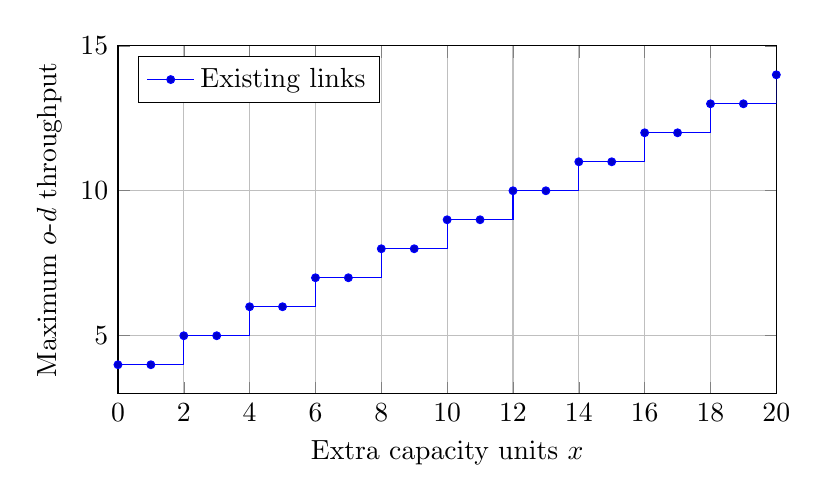
\begin{tikzpicture}
\begin{axis}[width=0.82\textwidth,height=6cm,grid=major,
 xlabel={Extra capacity units $x$},ylabel={Maximum $o$-$d$ throughput},xmin=0,xmax=20,ymin=3,ymax=15,
 xtick={0,2,...,20},legend pos=north west]
\addplot+[const plot,mark=*,mark size=1.4pt] coordinates {(0,4) (1,4) (2,5) (3,5) (4,6) (5,6) (6,7) (7,7) (8,8) (9,8) (10,9) (11,9) (12,10) (13,10) (14,11) (15,11) (16,12) (17,12) (18,13) (19,13) (20,14)};
\addlegendentry{Existing links}
\end{axis}
\end{tikzpicture}
